\documentclass[11pt,a4paper,oldfontcommands]{memoir}
\usepackage{ctex}
\usepackage[utf8]{inputenc}
\usepackage[T1]{fontenc}
\usepackage{microtype}
\usepackage[dvips]{graphicx}
\usepackage{xcolor}
\definecolor{linkColor}{RGB}{0, 153, 230}

\usepackage{times}
\usepackage{listings}
\usepackage{courier}
\lstset{
    columns=fixed,       
    %numbers=left,                                        % 在左侧显示行号
    frame=none,                                          % 不显示背景边框
    backgroundcolor=\color[RGB]{245,245,244},            % 设定背景颜色
    keywordstyle=\color[RGB]{40,40,255},                 % 设定关键字颜色
    %numberstyle=\footnotesize\color{darkgray},           % 设定行号格式
    commentstyle=\color[RGB]{0,96,96},                   % 设置代码注释的格式
    stringstyle=\rmfamily\slshape\color[RGB]{128,0,0},   % 设置字符串格式
    showstringspaces=false,                              % 不显示字符串中的空格
    language=c++,                                        % 设置语言
    basicstyle=\small\ttfamily
}

\usepackage[
breaklinks=true,colorlinks=true,
%linkcolor=blue,urlcolor=blue,citecolor=blue,% PDF VIEW
linkcolor=black,urlcolor=black,citecolor=black,% PRINT
bookmarks=true,bookmarksopenlevel=2]{hyperref}

\usepackage{amsmath}
\usepackage{hyperref}

\usepackage{geometry}
% PDF VIEW
\geometry{total={210mm,297mm},
left=25mm,right=25mm,%
bindingoffset=0mm, top=25mm,bottom=25mm}

% PRINT
%\geometry{total={210mm,297mm},
%left=20mm,right=20mm,
%bindingoffset=10mm, top=25mm,bottom=25mm}

\OnehalfSpacing
\chapterstyle{bianchi}
\setsecheadstyle{\Large\bfseries\sffamily\raggedright}
\setsubsecheadstyle{\large\bfseries\sffamily\raggedright}
\setsubsubsecheadstyle{\bfseries\sffamily\raggedright}

\pagestyle{plain}
\makepagestyle{plain}
\makeevenfoot{plain}{\thepage}{}{}
\makeoddfoot{plain}{}{}{\thepage}
\makeevenhead{plain}{}{}{}
\makeoddhead{plain}{}{}{}
\maxsecnumdepth{subsection} % chapters, sections, and subsections are numbered
\maxtocdepth{subsection} % chapters, sections, and subsections are in the Table of Contents

\graphicspath{ {./figure/} }

\begin{document}
\thispagestyle{empty}
{
\sffamily
\centering
{\LARGE
Introduction To 3D Game Programming with DirectX12 - 习题解
}

\vspace{3.5cm}
(草稿)\\
\clearpage
\tableofcontents*
\clearpage


\chapter*{6.13 习题}
%---------- 1 ----------------
\begin{flushleft}
1. 写出下面顶点结构的 D3D12\_INPUT\_ELEMENT\_DESC 数组:
\end{flushleft}
\begin{lstlisting}
struct Vertex
{
    XMFLOAT3 Pos;
    XMFLOAT3 Tangent;
    XMFLOAT3 Normal;
    XMFLOAT2 Tex0;
    XMFLOAT2 Tex1;
    XMCOLOR  Color;
};
\end{lstlisting}
\begin{flushleft}
答:\\
\end{flushleft}
\begin{lstlisting}
std::vector<D3D12_INPUT_ELEMENT_DESC> mInputLayout;
mInputLayout = {
    { "POSITION", 0, DXGI_FORMAT_R32G32B32_FLOAT, 0, 0, 
                  D3D12_INPUT_CLASSIFICATION_PER_VERTEX_DATA, 0 },
    { "TANGENT",  0, DXGI_FORMAT_R32G32B32_FLOAT, 0, 12, 
                  D3D12_INPUT_CLASSIFICATION_PER_VERTEX_DATA, 0 },
    { "NORMAL",   0, DXGI_FORMAT_R32G32B32_FLOAT, 0, 24, 
                  D3D12_INPUT_CLASSIFICATION_PER_VERTEX_DATA, 0 },
    { "TEXCOORD", 0, DXGI_FORMAT_R32G32_FLOAT, 0, 36, 
                  D3D12_INPUT_CLASSIFICATION_PER_VERTEX_DATA, 0 },
    { "TEXCOORD", 1, DXGI_FORMAT_R32G32_FLOAT, 0, 44, 
                  D3D12_INPUT_CLASSIFICATION_PER_VERTEX_DATA, 0 },
    { "COLOR",    0, DXGI_FORMAT_R8G8B8A8_UINT, 0, 52, 
                  D3D12_INPUT_CLASSIFICATION_PER_VERTEX_DATA, 0 }
};
\end{lstlisting}

%---------- 2 ----------------
\begin{flushleft}
~\\
2. 重写Box DEMO,这次使用 2 个顶点缓冲区(2个输入槽)给管道提供顶点数据。一个缓冲区存储位置元素,另一个存储存储颜色元素。下面给定两个分开的顶点数据结构:\\
\end{flushleft}
\begin{lstlisting}
struct VPosData
{
    XMFLOAT3 Pos;
};

struct VColorData
{
    XMFLOAT4 Color;
};
\end{lstlisting}
\begin{flushleft}
位置元素挂在输入槽0上,颜色元素挂在输入槽1上。此外还需注意 D3D12\_INPUT\_ELEMENT\_DESC::AlignedByteOffset 对于两个元素来说都是0;然后使用 ID3D12CommandList::IASetVertexBuffers 方法来将缓冲区绑定到槽0和槽1。然后,Direct3D将使用来自不同输入槽的元素来组合顶点。 这可以用作优化。 例如,在阴影映射算法中,我们需要每帧绘制两次场景:一次从光源的角度(阴影传递),一次从主摄像头的角度(主传递)。 阴影传递仅需要位置数据和纹理坐标(对于经过alpha测试的几何体)。 因此我们可以将顶点数据分成两个槽:一个槽包含位置和纹理坐标,另一个槽包含其他顶点属性(例如,法线和切线矢量)。 现在我们可以轻松地仅在阴影传递所需的顶点数据中流动(位置和纹理坐标),从而为阴影传递节省数据带宽。 主渲染过程将使用两个顶点输入槽来获取所需的所有顶点数据。 为了提高性能,建议最小化用于小于或等于3的小数字的输入槽数。\\
\end{flushleft}
\begin{flushleft}
答:TODO
\end{flushleft}

%---------- 3 ----------------
\begin{flushleft}
3. 绘制以下图形:\\
\begin{itemize}
  \item 1. 一个点列表(point list),如图5.13a。
  \item 2. 一个线段条(line strip),如图5.13b。
  \item 3. 一个线段列表(line list),如图5.13c。
  \item 4. 一个三角条(triangle strip),如图5.13d。
  \item 5. 一个三角列表(triangle list),如图5.14a。
\end{itemize}
答: \\
\begin{itemize}
  \item 1. 修改 BoxApp::Draw 方法:\\
  \begin{lstlisting}
  // D3D11_PRIMITIVE_TOPOLOGY_TRIANGLELIST 改为 D3D11_PRIMITIVE_TOPOLOGY_POINTLIST
  mCommandList->IASetPrimitiveTopology(D3D11_PRIMITIVE_TOPOLOGY_POINTLIST);
  \end{lstlisting}
  \item 2. 同 1 改为 D3D11_PRIMITIVE_TOPOLOGY_LINESTRIP 即可
  \item 3. 同 1 改为 D3D11_PRIMITIVE_TOPOLOGY_LINELIST 即可
  \item 4. 同 1 改为 D3D11_PRIMITIVE_TOPOLOGY_TRIANGLESTRIP 即可
  \item 5. 同 1 改为 D3D11_PRIMITIVE_TOPOLOGY_TRIANGLELIST 即可
\end{itemize}

\end{flushleft}

%---------- 4 ----------------
\begin{flushleft}
4. 构造金字塔的顶点和索引列表,如图\ref{fig:6-8}所示,并绘制它。 将基顶点设为绿色和顶上顶点设为红色。\\
答:TODO
\end{flushleft}
\begin{figure}[h]
    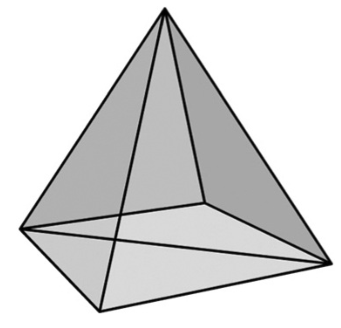
\includegraphics[width=\textwidth]{6-8}
    \centering
    \caption{金字塔三角形}
    \label{fig:6-8}
\end{figure}
%---------- 5 ----------------
\begin{flushleft}
5. 运行“Box” DEMO,并回想一下我们仅在顶点指定颜色。 解释如何为三角形上的每个像素获取像素颜色。
\end{flushleft}


%---------- 6 ----------------
\begin{flushleft}
6. 修改 Box Demo, 在转换为世界空间之前将以下变换应用于顶点着色器中的每个顶点。
\end{flushleft}
\begin{lstlisting}
vin.PosL.xy += 0.5f*sin(vinL.Pos.x)*sin(3.0f*gTime);
vin.PosL.z *= 0.6f + 0.4f*sin(2.0f*gTime);
\end{lstlisting}
\begin{flushleft}
您需要添加一个gTime常量缓冲区变量; 此变量对应于当前的 GameTimer::TotalTime() 值。 使用正弦函数周期性地扭曲顶点来将时间通过顶点动画来展现。
\end{flushleft}

%---------- 7 ----------------
\begin{flushleft}
7. 将箱(box)和金字塔的顶点(练习4)合并到一个大的顶点缓冲区中。 还将框和金字塔的索引合并到一个大索引缓冲区中(但不更新索引值)。 然后使用 ID3D12CommandList::DrawIndexedInstanced 的参数逐个绘制框和金字塔。 使用世界变换矩阵,使框和金字塔在世界空间中不相交。
\end{flushleft}

%---------- 8 ----------------
\begin{flushleft}
8. 通过在线框(wireframe)模式下渲染多维数据集来修改Box演示。
\end{flushleft}

%---------- 9 ----------------
\begin{flushleft}
9. 修改Box演示, 禁用背面剔除(D3D12\_CULL\_NONE); 也尝试剔除正面而不是背面(D3D12\_CULL\_FRONT)。 以线框(wireframe)模式输出结果,以便您可以更轻松地查看差异。
\end{flushleft}

%---------- 10 ----------------
\begin{flushleft}
10. 如果顶点内存很重要,那么从128位颜色值减少到32位颜色值可能是值得的。修改“Box”演示 在顶点结构中使用32位颜色值而不是128位颜色值。 您的顶点结构和相应的顶点输入描述将如下所示:\\
\end{flushleft}
\begin{lstlisting}
struct Vertex
{
    XMFLOAT3 Pos;
    XMCOLOR Color;
}

D3D12_INPUT_ELEMENT_DESC vertexDesc[] = {
    {“POSITION”, 0, DXGI_FORMAT_R32G32B32_FLOAT, 0, 0, 
                 D3D12_INPUT_PER_VERTEX_DATA, 0},
    {“COLOR”,    0, DXGI_FORMAT_B8G8R8A8_UNORM, 0, 12,
                 D3D12_INPUT_PER_VERTEX_DATA, 0}
};
\end{lstlisting}
\begin{flushleft}
我们使用 DXGI\_FORMAT\_B8G8R8A8\_UNORM 格式(8位红色,绿色,蓝色和alpha)。 此格式对应于常见的32位图形颜色格式ARGB,但 DXGI\_FORMAT 符号以小端表示法列出它们在内存中出现的字节。 在little-endian中,多字节(multi-byte)数据字(word)的字节从最低有效字节写入最高有效字节,这就是为什么 ARGB 在内存中出现为 BGRA,其中最小内存地址处的最低有效字节和最高有效字节为 最高的内存地址。
\end{flushleft}

%---------- 11 ----------------
\begin{flushleft}
11. 思考下面 C++ 顶点结构:
\end{flushleft}
\begin{lstlisting}
struct Vertex
{
    XMFLOAT3 Pos;
    XMFLOAT4 Color;
};
\end{lstlisting}
\begin{itemize}
  \item 1. 输入布局描述顺序是否需要匹配顶点结构顺序? 也就是说,以下顶点声明是否适用于此顶点结构? 做一个实验来找出答案。 然后给出你为什么认为它有效或无效的推理。
  \begin{lstlisting}
  D3D11_INPUT_ELEMENT_DESC vertexDesc[] =
  {
      {“COLOR”,    0, DXGI_FORMAT_R32G32B32A32_FLOAT, 0, 12,
                   D3D11_INPUT_PER_VERTEX_DATA, 0},
      {“POSITION”, 0, DXGI_FORMAT_R32G32B32_FLOAT, 0, 0,
                   D3D11_INPUT_PER_VERTEX_DATA, 0}
  };
  \end{lstlisting}
  \item 2. 相应的顶点着色器结构顺序是否需要匹配 C++ 顶点结构顺序? 也就是说,以下顶点着色器结构是否与上述 C++ 顶点结构一起使用? 做一个实验来找出答案。 然后给出你为什么认为它有效或无效的推理。
  \begin{lstlisting}
  struct VertexIn
  {
      float4 Color : COLOR;
      float3 Pos   : POSITION;
  };
  \end{lstlisting}
\end{itemize}

%---------- 12 ----------------
\begin{flushleft}
12. 将视口(viewport)设置为后缓冲区(back buffer)的左半部分。
\end{flushleft}

%---------- 13 ----------------
\begin{flushleft}
13. 使用剪刀测试来剔除以后缓冲区为中心的矩形外的所有像素,宽度为mClientWidth/2,高度为 mClientHeight/2。 请记住,您还需要使用光栅化器状态组启用剪刀测试。
\end{flushleft}

%---------- 14 ----------------
\begin{flushleft}
14. 像素着色器颜色色调。 使用常量缓冲区为颜色随时间变化。 使用平滑缓动功能。 在顶点着色器和像素着色器中执行此操作。
\end{flushleft}

%---------- 15 ----------------
\begin{flushleft}
15. 修改 Box DEMO 中的像素着色器为如下形式:
\end{flushleft}
\begin{lstlisting}
float4 PS(VertexOut pin) : SV_Target
{
    clip(pin.Color.r - 0.5f);
    return pin.Color;
}
\end{lstlisting}
\begin{flushleft}
运行程序并猜测内置 clip 方法的作用。
\end{flushleft}

%---------- 16 ----------------
\begin{flushleft}
修改 Box 演示中的像素着色器,以在插值顶点颜色和通过常量缓冲区指定的 gPulseColor 之间平滑脉冲。 您还需要更新应用程序端的常量缓冲区。 HLSL代码中的常量缓冲区和像素着色器应如下所示:
\end{flushleft}
\begin{lstlisting}
cbuffer cbPerObject : register(b0)
{
    float4x4 gWorldViewProj;
    float4 gPulseColor;
    float gTime;
};

float4 PS(VertexOut pin) : SV_Target
{
    const float pi = 3.14159;

    // Oscillate a value in [0,1] over time using a sine functio.
    float s = 0.5f*sin(2*gTime - 0.25f(pi) + 0.5f;

    // Linearly interpolate between pin.Color and gPulseColor based on
    // parameter s.
    float4 c = lerp(pin.Color, gPulseColor, s);
    return c;
}
\end{lstlisting}
\begin{flushleft}
gTime 变量对应于 GameTimer::TotalTime() 的值。
\end{flushleft}

\chapter{7.9 习题}
%---------- 1 ----------------
\begin{flushleft}
1.修改“Shapes”演示以使用 GeometryGenerator::CreateGeosphere 而不是 GeometryGenerator::CreateSphere。 尝试使用0,1,2和3细分级别。\\
\end{flushleft}

%---------- 2 ----------------
\begin{flushleft}
2.修改“Shapes”演示以使用十六个根常量来设置每个对象的世界矩阵而不是描述符表。\\
\end{flushleft}

%---------- 3 ----------------
\begin{flushleft}
3.在DVD上,有一个名为 Models/Skull.txt 的文件。 该文件包含图\ref{fig:7-11}中渲染头骨所需的顶点和索引列表。 使用文本编辑器(如记事本)研究文件,并修改“形状”演示以加载和渲染头骨网格。\\
\end{flushleft}

\begin{figure}[h]
    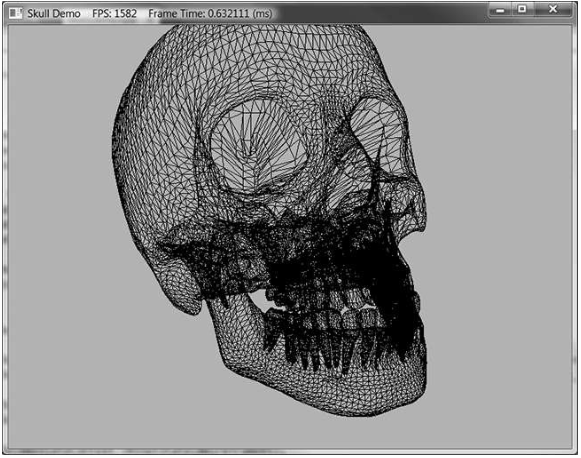
\includegraphics[width=\textwidth]{7-11}
    \centering
    \caption{练习3的渲染输出}
    \label{fig:7-11}
\end{figure}

\end{document}
